\newpage
\section{3 Dimensional Analysis}
\noindent This section is an extended analysis of the 2 dimensional analyses which intended to explore and analyse the 3 dimensional flow feature. It was surmised that the 3 dimensional flow offer a complex flow behaviour that may significantly affect overall performance of an undertray. This part of the paper will be divided into 3D open-flow and undertray prototype with bluff body analyses.


\subsection{3D Open-Flow}
\subsubsection{Overview}
This analysis is an extension of 3 dimensional analysis of 2D open-flow. The purpose of this analysis to investigate further the flow features of an undertray in 3 dimensional manner which plausibly affect its performance based on similar variable as previous analyses.

\subsubsection{Geometry and Mesh generation}
An identical 2D sketch from geometry 3 - 2D open flow was used, which then extruded to 1 meter of thickness with skirt on both side of the rear diffuser. The skirts were used to improve flow isolation  and generate corner vortices which help to improve flow attachment at the diffuser region. Fences were also added on the next analyses to investigate the effect of vortex generator on downforce generation. Illustration of both geometries can be seen on figure \ref{fig:3D_OF_GEOM} below.  

\begin{figure}[!h]
    \centering
    \noindent\makebox[\textwidth]{
    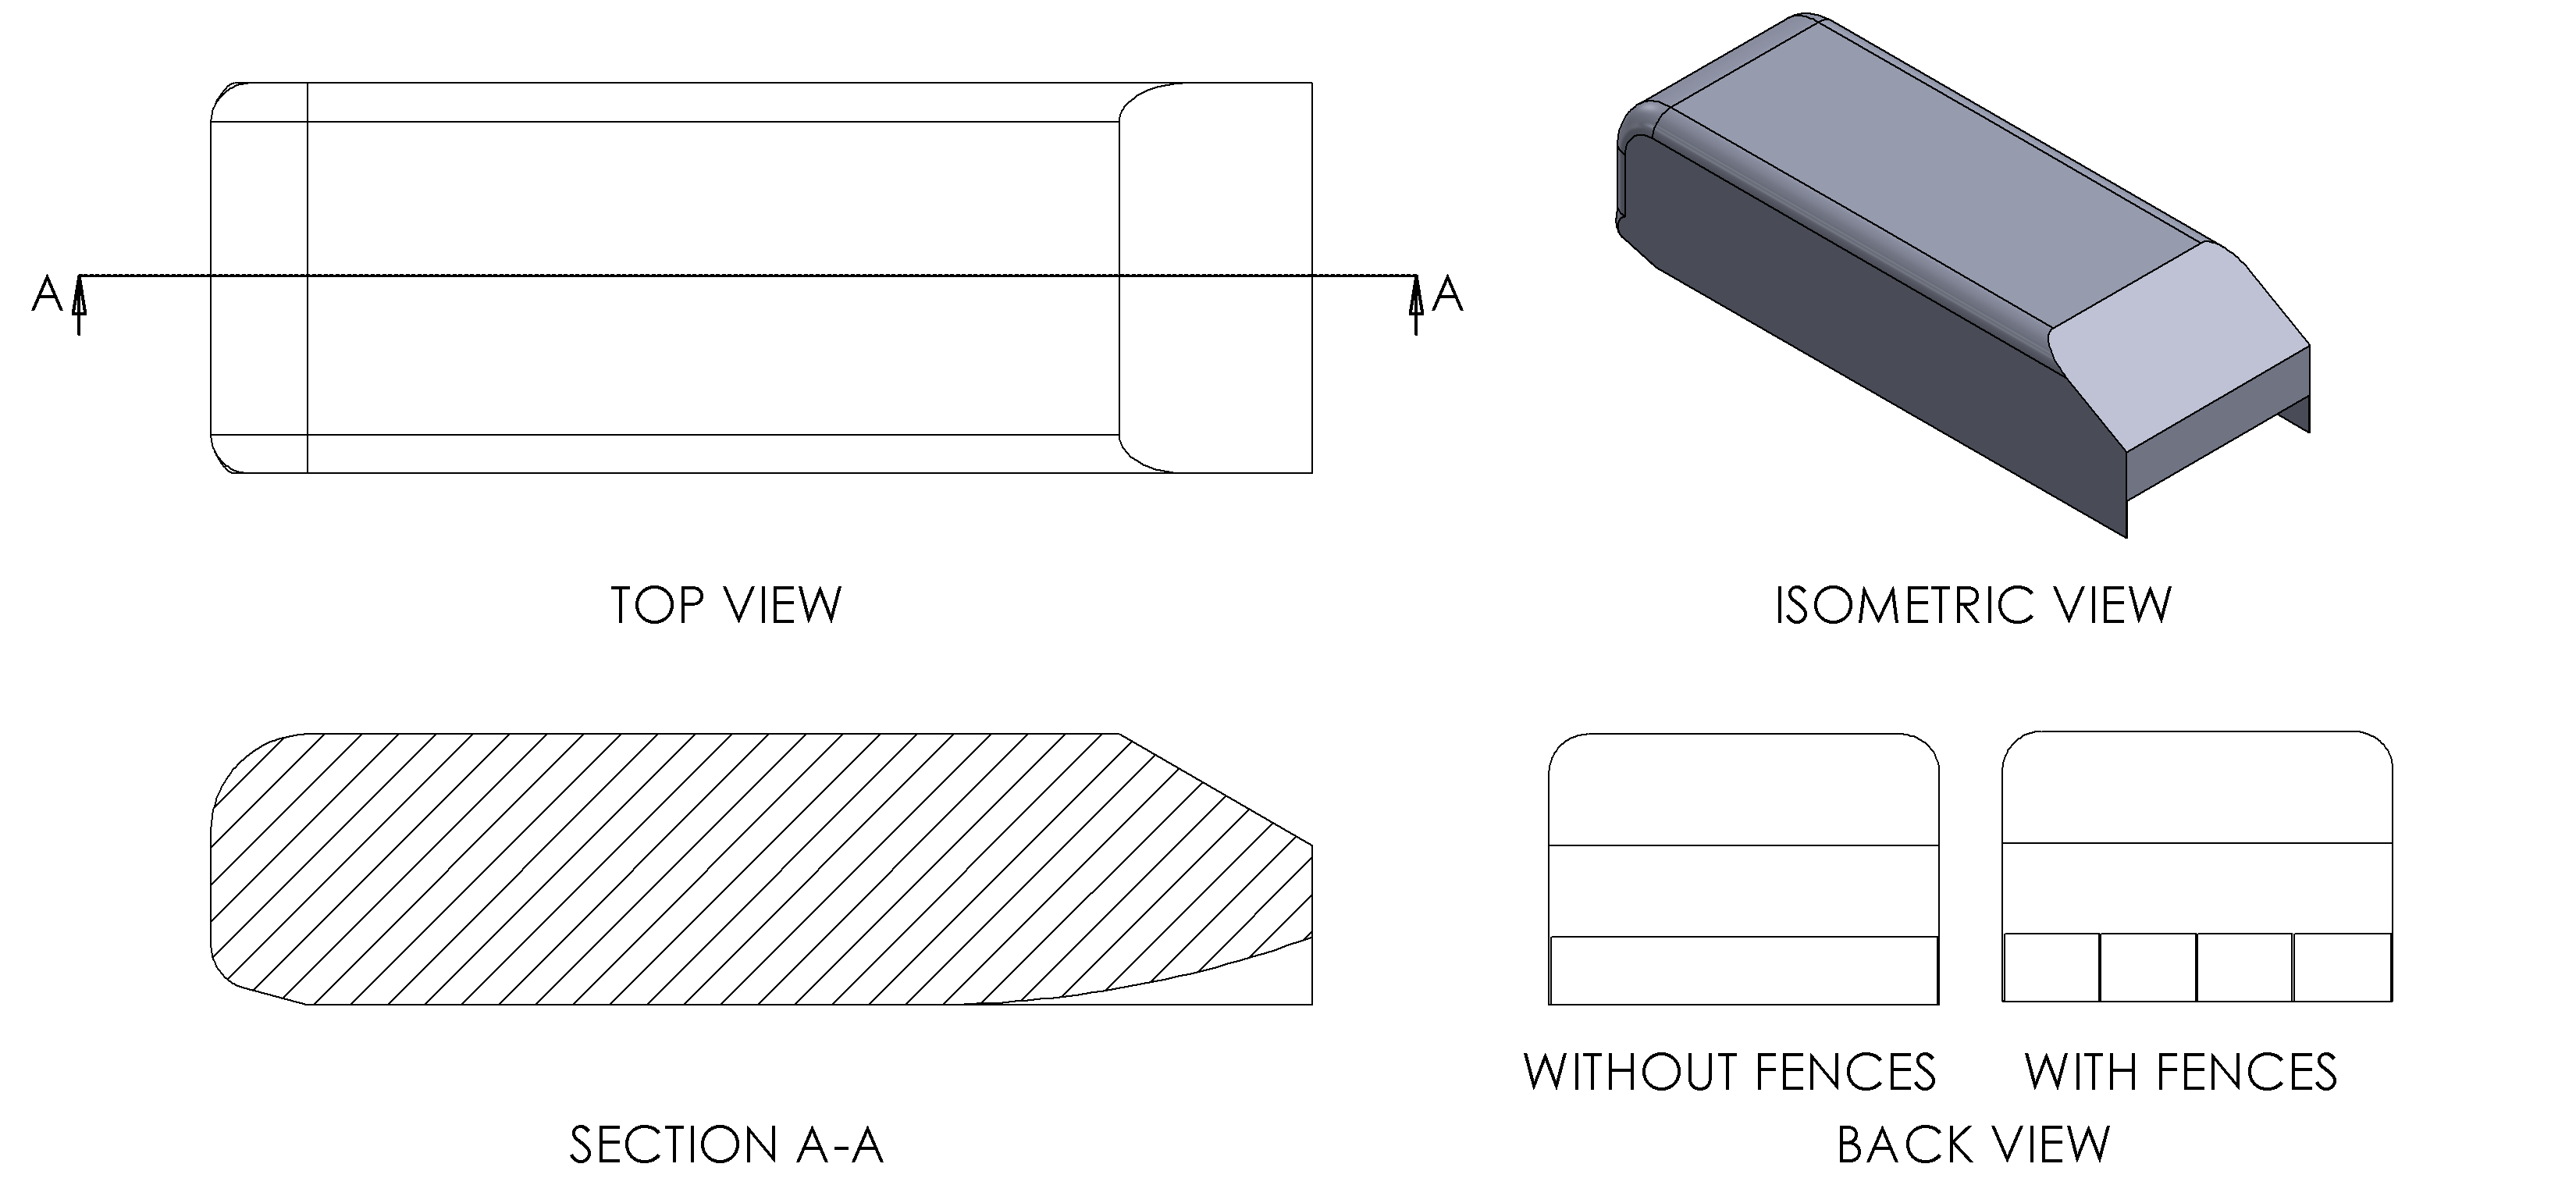
\includegraphics[width=0.8\textwidth]{Figures/3D_OF/3D_OF_D.PNG}}
    \caption{Geometry generated for 3D open-flow analysis.}
    \label{fig:3D_OF_GEOM}
\end{figure}

\noindent The geometry then was imported to the design modeller where fluid domain and body of influence were made. The fluid flow was made with 12 meters behind, 5 meters forward, 2 meters top, 0.03 meters bottom, and 1.5 meters wide. Due to the body's symmetry, partial model was used to create fluid domain to compress the number of mesh. Body of influence (BOI) with dimension of  6 $\times$1 $\times$ 7 meters were created using box feature around the body to improve the mesh quality and capture the flow features of the surrounding.  

\noindent A hybrid mesh was used which comprise of tetrahedron and triangular prisms which construct 20 inflation layer of triangular prism near the wall with y$^+$=1.  Mesh element size of 0.8 meters and 0.02 meters of BOI generated 1.3 to 1.5 millions of mesh elements for this analysis. Mesh quality of this section is considerably acceptable with average skewness of 1.9 and aspect ratio of 80-90, however, an extreme jump size in cell between the inflation layer and far-field fluid domain  considered as not ideal. Detailed illustration of the fluid domain and the mesh can be seen on figure X Appendix C.

\subsubsection{Results and Discussions}
Due to the nature of the mesh, k-$\omega$ SST model was used throughout this analysis to take advantage of the feature of this transport model \cite{Ansys2006ModelingFlows}. Analyses will be grouped into three geometries which are diffuser angle variables with no inlet angle, diffuser variables with 10 degrees inlet angle, inlet angle variable with 10 degrees diffuser angle, and variable diffuser angle with three fences applied.  Figure \ref{fig:3D_OF_PLOT_COMPARE_ALL} below shows comparison of lift and drag between all variables.

\begin{figure}[htb!]
    \centering
    \noindent\makebox[\textwidth]{
    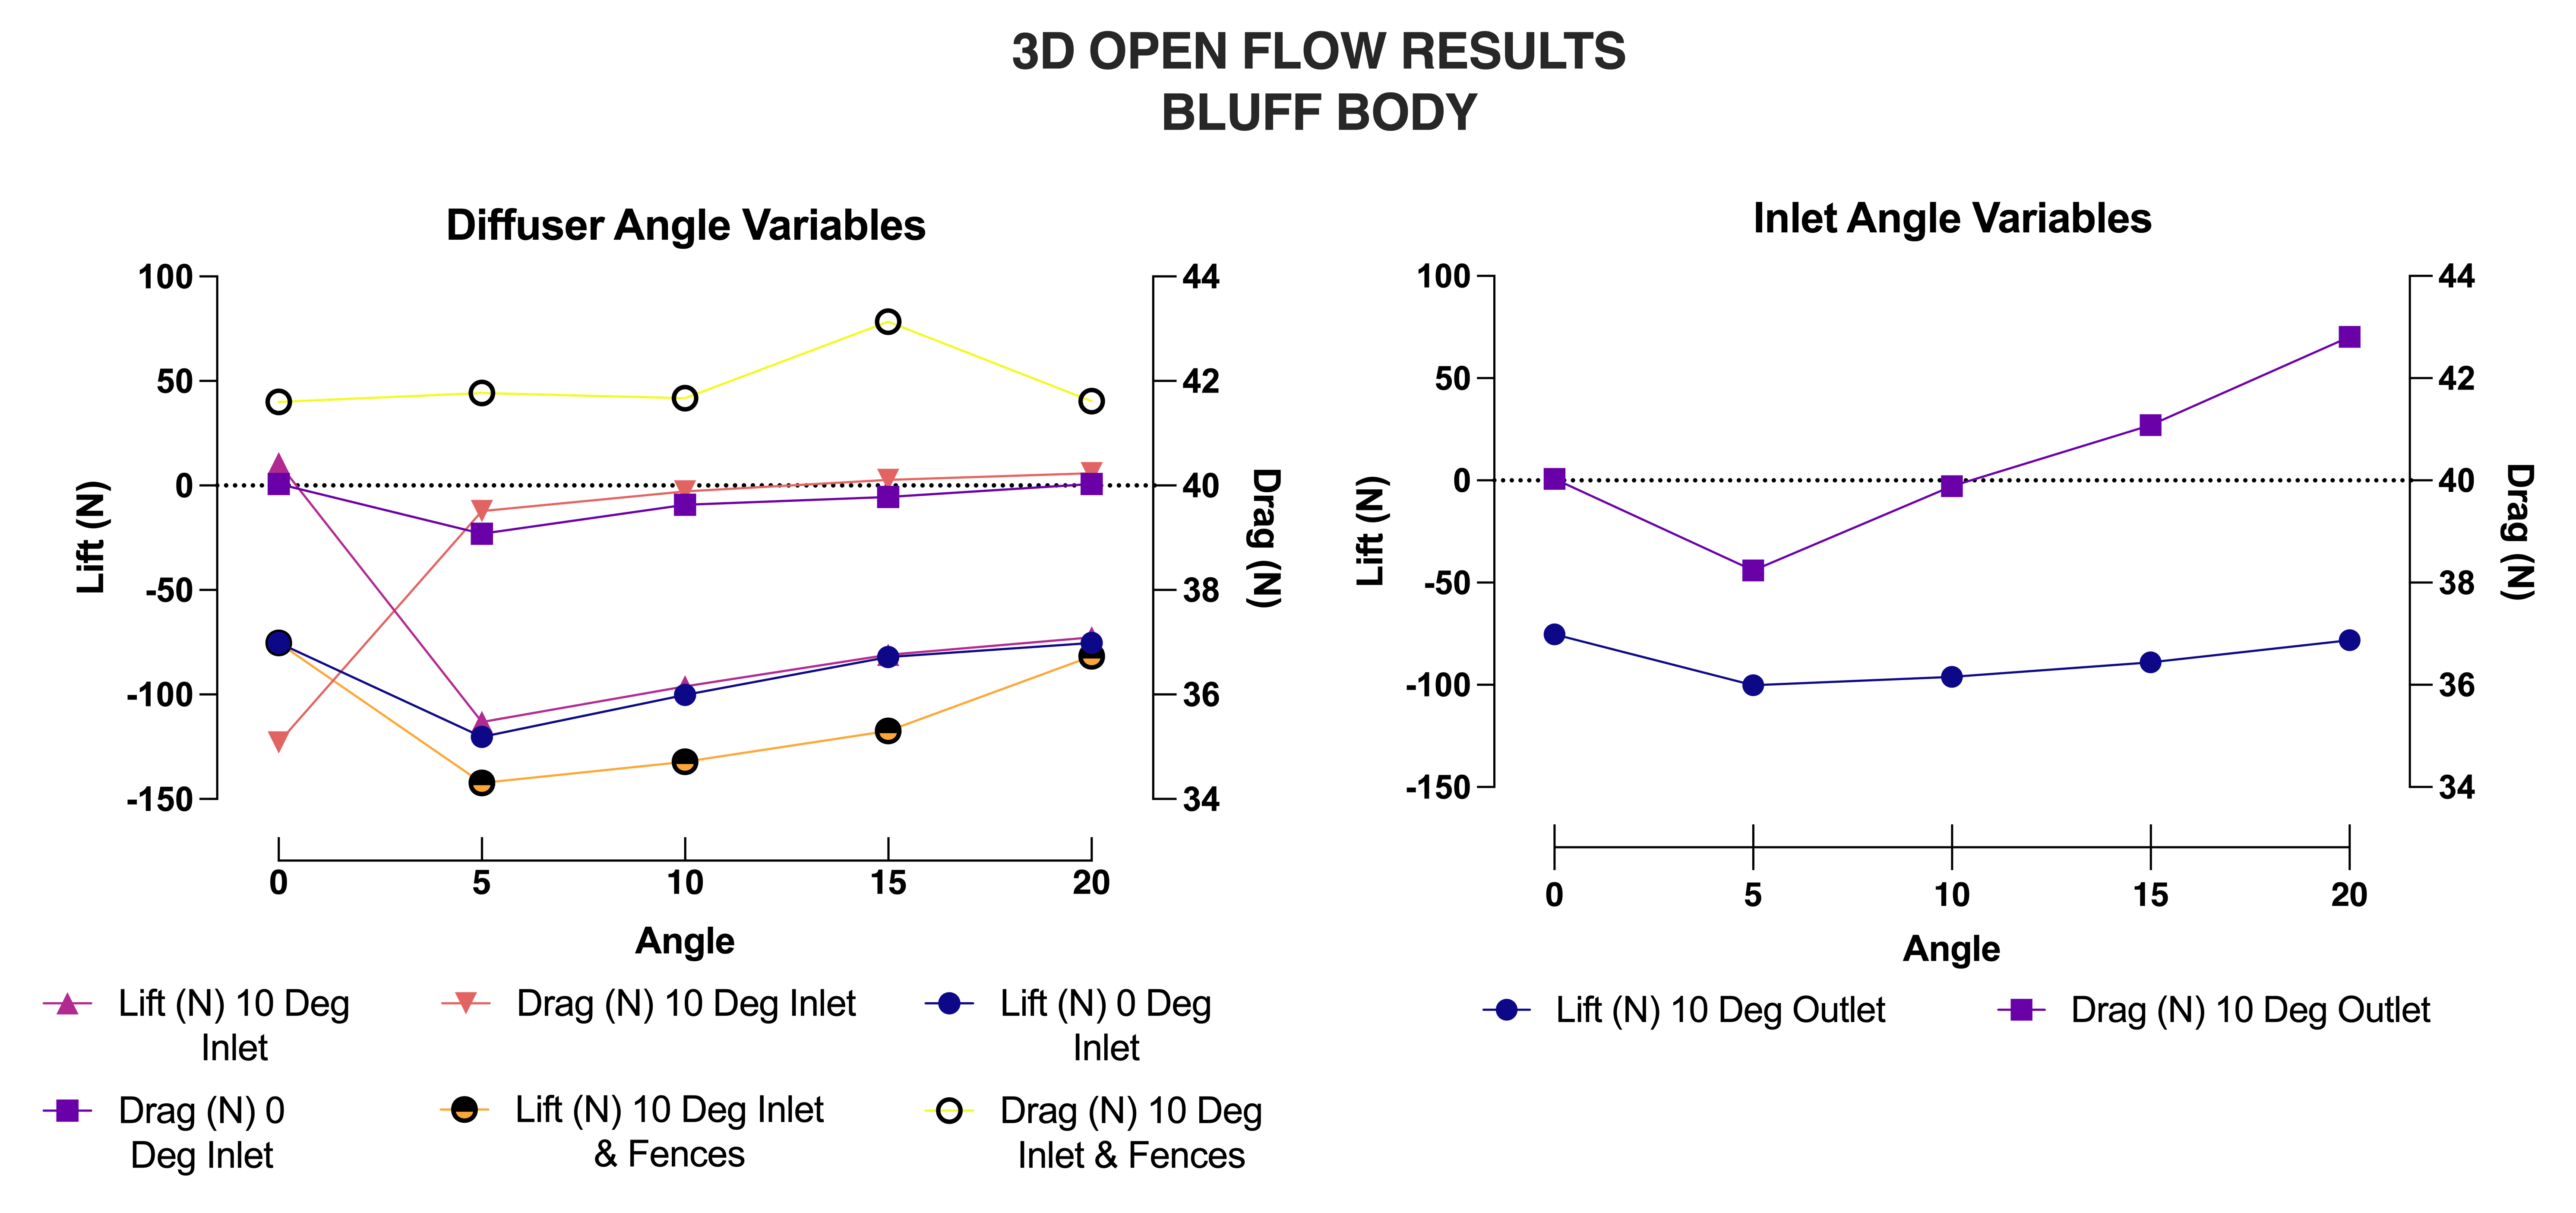
\includegraphics[width=1\textwidth]{Figures/Graph/3D_OF.png}}
    \caption{Lift and drag variation of diffuser (left) and inlet (right) angle for all geometry configurations..}
    \label{fig:3D_OF_PLOT_COMPARE_ALL}
\end{figure}
\noindent The value of lift and drag shown represent half of the bluff body as computed. Once more, similar trend emerged compared to 2D open flow geometry 4 means the 2D bluff body on this case can be deduced as representation of the 3D analysis.  The trend shows increase in downforce at 5 degrees diffuser angle then followed by linear downforce reduction up to 20 degrees.  In comparison with 2D open-flow analysis, the average downforce of this analysis is significantly lower. This is due to the nature of the analysis that allows the accelerated flow in the undertray to be affected by the flow surrounding the body compared to the 2D open-flow where the flow on the undertray  is solely affected by the flow. This cause the lower pressure region in the undertray to suck in the air from surrounding,  reducing the effectiveness of the flow acceleration underneath, hence lower downforce. This phenomenon is illustrated on figure X below. %show the flow region from outside affecting the flow inside.

\noindent Comparing the lift and drag for diffuser variable with or without inlet angle, the graph indicates an identical results except the one at 0 degrees.  There is a noticeable drop in downforce and drag (however insignificant) which plausibly due to the absent of the diffuser. A presence of well-designed diffuser is important to slowly expand the flow and allows the jet flow to stay attached to the diffuser's. Moreover, the presence of diffuser allows the side-skirts to generate corner vortices which help the flow to attached, hence increase the overall downforce. The vortex generation phenomenon will be explained further later in this paper. %shows the vortex on the side of the diffuser

\noindent On the other hand the lift and drag reached it's lowest at 5 degrees inlet angle and followed by its reduction up to 20 degrees. %why does the the increase of inlet angle increase the drag and drop the lift?.

\noindent The next analysis will include fences to generate corner vortices and investigate its effect on the undertray's performance. It can be seen from figure X, that additional 3 fences on the diffuser is proven to increase the overall downforce and drag of the body. As the air sucked in from the side of the skirt, a corner vortex is formed due to difference in pressure. This vortex allows the flow from the undertray's throat to stick on the wall which indicated by the x-wall shear gradient shown on figure x below. This indi









\subsection{3D Undertray}

\subsubsection{Overview}
\subsubsection{Geometry and Mesh Generation}
\subsubsection{Results and Discussion}
